\documentclass{article}
\usepackage{lmodern} % Latin Modern Font
\usepackage[T1]{fontenc}
\usepackage{amsfonts} % \mathbb
\usepackage[margin=0.5in]{geometry}
\usepackage[utf8]{inputenc}
\usepackage{graphicx}
% \graphicspath{{images/}}
\usepackage[backend=biber]{biblatex}
\usepackage{amsmath}
\usepackage[makeroom]{cancel}

% \usepackage{auto-pst-pdf}

% \usepackage{hyperref}
% \usepackage{hypcap}
% \DeclareMathOperator{\sign}{sign}
% \hypersetup{
%   colorlinks=true, 
%   allcolors=black,
%   pdfauthor={Carlos Henrique Tarjano Santos},
%   pdftitle={Robust Digital Envelope Estimation Via Geometric Properties of an Arbitrary Real Signal}
% }

\bibliography{bibli}

\usepackage{authblk}
\title{Robust Digital Envelope Estimation Via Geometric Properties of an Arbitrary Real Signal}
\author[1]{Carlos Henrique Tarjano Santos}
\author[2]{Valdecy Pereira}
\affil[1]{(corresponding author, carlostarjano@id.uff.br) Department of Production Engineering, Universidade Federal Fluminense, Rua Passo da Pátria, 156, Campus Praia Vermelha, Bloco D - sala 309, São Domingos, Niterói, RJ, Brasil, CEP: 24.210-240}
\affil[2]{Department of Production Engineering, Universidade Federal Fluminense, Rua Passo da Pátria, 156, Campus Praia Vermelha, Bloco D - sala 309, São Domingos, Niterói, RJ, Brasil, CEP: 24.210-240}

\begin{document}

\maketitle

\begin{abstract}

\end{abstract}

{\bf Keywords:} DSP, alpha-shapes, envelope detection, discrete curvature estimation


\section{Introduction}



We aim to exploit redundancies in the constitution of a discrete sound wave to formulate an alternative, more compact and thus easier to analyse, representation. Implicit in this affirmation is the somewhat loose assumption that the wave considered is reasonably well behaved, in the sense that redundancies exist to be identified. In contrast with \textcite{2019TarjanoNeuro}, we don't require the signal to be strictly harmonic.

We aim in providing a method that, with minimal manual interference, is able to reduce a digital wave to a more compact and meaningful representation.


\section{Methodology}
Conceptually, one can think of the procedure here presented as a way to represent discrete, pitched, signal with a set of 3 tuples. Those tuples are composed, to describe them loosely, of a polynomial description of the envelope of the signal, that dictates the outer shape of the wave, or the volume of the sound as a function of time; another polynomial description, but this time for the (pseudo)-cycles of the wave, meant to represent the shape of each pseudo cycle of the signal, and a description of the beginning of each said pseudo cycle, and thus the end of the preceding one.

This aids in putting in perspective the broad strokes of the algorithm.


\subsection{Pseudo Cycles}

This work proposes the pseudo cycle as the building block of a discrete wave, assuming its parametric shape to be constant throughout the space of the digital signal; in order words, the adjective pseudo is used because the two other descriptions of the wave, namely, the envelope and the length of the pseudo cycles act into the pseudo cycles shape itself, modifying it in function of the time.

This is a simplification, as many factors are known to influence the shape pseudo cycles of an arbitrary wave throughout time, as is the case of the decaying high frequencies in a rigid string, for example. % TODO Those factors will be eventually accounted for

Using the envelope detection algorithm presented in \textcite{2020TarjanoRobust} one can identify the frontiers, both positive and negative, of a digital signal: Those are, ideally, respectively composed of the maxima and minima of each pseudo-cycle of a discrete signal. 

If we disconsider inaccuracies we could use either one of the frontiers to infer the exact position, wavelength and amplitude of each pseudo-cycle and to, provided that the shape of the wave is also known, reconstruct the original wave with those pieces of information. Consider, for example, the digital signal presented in figure \ref{fig:signalenvelope}
and the extracted frontiers; the signal is an example of the voice of an alto singer, with its frontiers in black.

\begin{figure}[ht!]
  \centering
     \includegraphics{images/01signalenvelope.pdf}
  \caption{A discrete wave of the singing voice of an alto singer. The black lines are the frontiers; in the detail view, it can be seen that each region between two diamonds comprises a pseudo-cycle, as defined by the points belonging to the upper frontier. Similarly, two adjacent squares delimitate a pseudo-cycle, from the standpoint of the lower frontier.}
  \label{fig:signalenvelope}
\end{figure}

It can be seen that both frontiers provide approximately the same information about the location of each pseudo-cycle, albeit with a phase difference between them. As the original algorithm proposed in \textcite{2020TarjanoRobust} is meant for envelope detection, maxima or minima that lies close to the already established frontiers are sometimes neglected, without significant impact in the envelope extracted.

This can be seen in the discrete representation of the sound of the key 33 of a grand piano in figure \ref{fig:frontiergaps}, as the black squares and diamonds: intuitively, one can see that some local maxima and minima are missing, compromising the identification of all pseudo cycles. For our purposes, however, it is beneficial to accurately identify as many local maxima and minima, and hence pseudo cycles, as possible, as the impact on the shape of a pseudo cycle is significant.

We are going to assume that all the local extremes identified by the envelope detection algorithm are indeed correct; albeit not being strictily accurate, this approximation is very reasonable and simplifies further steps immensely, as we now need only to idenfity pseudo cycles with periods $ T $, that is, the difference between two adjacent maxima or minima, that are significantly bigger than the average observed in the discrete wave, and identify their local maximum or minimum, respectively.

The result of this procedure can be seen ad the gray squares and diamonds in figure \ref{fig:frontiergaps}.

\begin{figure}[ht!]
  \centering
     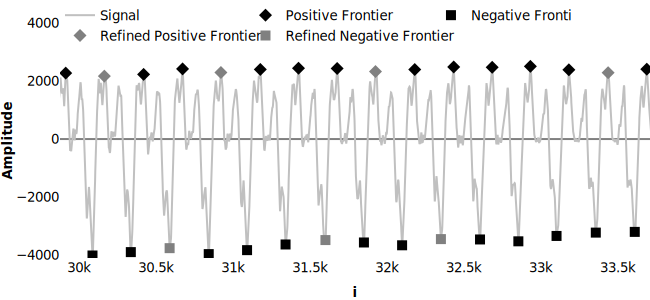
\includegraphics{images/02frontiergaps.pdf}
  \caption{Close-up view of a discrete signal representing the sound of the key 33 of a grand piano and its original positive and negative frontiers, in black, as well as the additional extrema identified during the refining process.}
  \label{fig:frontiergaps}
\end{figure}



% Consider, for example, the periodic discrete signal shown in the figure \ref{fig:periodicwave} below, consisting of the repetition of a cycle constructed from a simple sinusoid with gaussian noise added, where the maxima and the minima were highlighted.

% \begin{figure}[ht!]
%   \centering
%      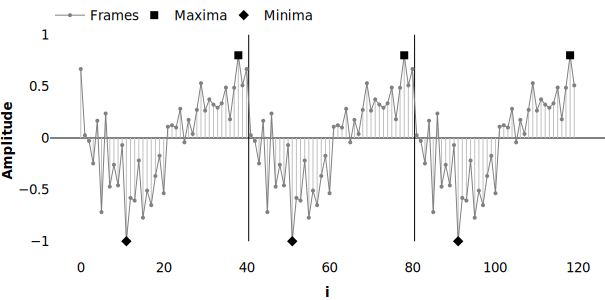
\includegraphics{07periodicwave.pdf}
%   \caption{Three Cycles, divided by the vertical lines, of a discrete periodic wave, with the maxima and minima highlighted}
%   \label{fig:periodicwave}
% \end{figure}

% The first thing we can observe from \ref{fig:periodicwave} is that there are three types of well defined points of interest in the cycle of an arbitrary periodic discrete wave of the form $ f(x) = f(x + P) \forall x \in D(f) $, where $ D $ is the domain of the function $ f $: The extreme points, that is, the maxima and minima, and the zeroes.

% It is easy to see that if we choose to plot the frame of ocurrence of those points as a function of their cardinality, breaking ties arbitrarily and consistently, we will invariably have a straight line of the form $ y = a x + b $, in the case of strictily periodic waves, with the slope related to the dominant frequency, and the intercept related to the concept of phase.

% Also, we can argue that using the maxima, instead of the zeroes, brings some simplifications to the process, as the maxima are generally less abundant, and more directly well defined, both in the horizontal and vertical axes. The vertical difference of one of such points and the immediately adjacent one is the period $ T $ of the periodic wave.

% Two things about this straight line become, then, immeadiately apparent: the first is that unit in the vertical axis is $ i $, that is, the indices of the frames of the discrete wave, and the second is that $ x \in \mathbb{N} $. Also, we have that the slope of the line equation is $ a = \frac{y_{k+1} - y_{k}}{x_{k+1} - x_{k}} = T $.

% We can then rewrite the line equation as $ y_k = T x_k + b $

% % $ b = \frac{x_{k+1} y_{k} - x_{k} y_{k+1}}{x_{k+1} - x_{k}} $

% If we define the local frequency $ f $ of a discrete, periodic wave as the ratio between the number cycles of said wave and the number $ n $ of frames of that wave, we can, recalling that the period of a wave is the inverse of its frequency, obtain the dominant frequency of the wave by using the equation $ f = \frac{n}{T} = \frac{n}{a} $. Alternatively, the relation $ f = (\#F^\pm - 1) n / (F^\pm[-1] - F^\pm[0])$, where $ \#F^\pm $ denotes the cardinality of the frontier, while $ F^\pm[0] $ and $ F^\pm[-1] $ stand for the frontier's first and last item, respectively, could also be used.

% Similarly, it is simpler to obtain information about the phase of a periodic wave from the extremes. Keeping in mind that a phase shift of $ 2 \pi $ would shift the wave by one whole period and also that a wave with zero phase would have its first maximum at $ i = 0 $, we need only to multiply the ratio between the frame where the first maximum ocurred and the period by 
% $ 2 \pi $, as in the formula $ \phi = \frac{2 \pi F^+[0]}{T}$

% About the result above it is important to keep in mind that congruency with the results of the Fourier Transform is not guarateed, as the shape of an arbitrary wave and, consequently, the relative position of its maximum can depart considerably from the position of an ordinary sinusoid.

% By this token, it is more convenient to define the phase obtained from the negative frontier in terms of the one obtained with the use of the positive one; To achieve that, it is sufficient to infer the relative position of the maximum in relation to the minimum, and use that in the phase formula presented above.




\begin{figure}[ht!]
  \centering
     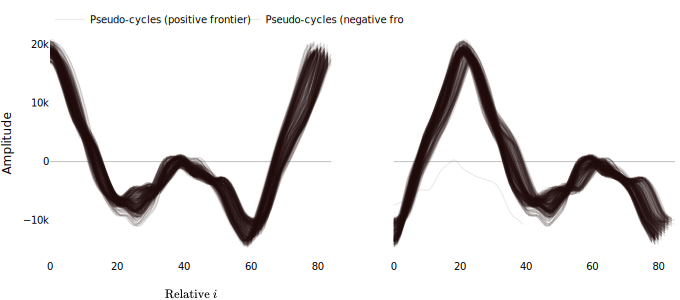
\includegraphics{02pcsraw-alto.pdf}
  \caption{Raw pseudo-cycles superimposed as defined by the positive and negative frontiers, for the alto singer signal.}
  \label{fig:pcrawalto}
\end{figure}

We can normalize the amplitude the pseudo-cycles between zero and one, by dividing each of them by their maximum. The lengths of each pseudo-cycle can be normalized with the use of the Fourier transform; to avoid any loss of data, we can use the maximum wavelength as the standard.

\begin{figure}[ht!]
  \centering
    %  \includegraphics[width=0.9\linewidth]{01signalenvelope}
     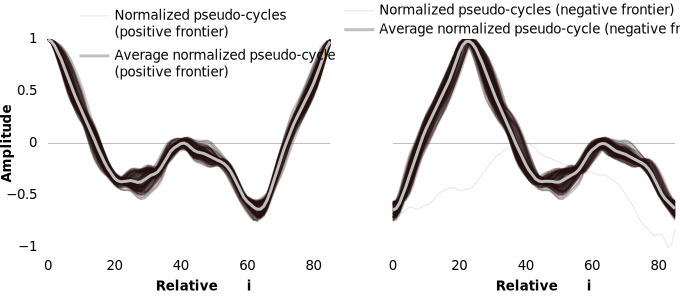
\includegraphics{03pcs-alto.pdf}
    % \def\svgwidth{\linewidth}
    %\input{01signalenvelope.pdf_tex}
  \caption{Normalized pseudo-cycles superimposed as defined by the positive and negative frontiers, for an alto singer signal, and the average of all normalized pseudo-cycles.}
  \label{fig:pcalto}
\end{figure}

Comparing figures \ref{fig:pcrawalto} and \ref{fig:pcalto} we note the effect of the normalization, as a means to reduce the variance of the pseudo-cycles, specially in the regions near the discontinuities. This will enable a more accurate approximation of the average wave.


\begin{figure}[ht!]
  \centering
    %  \includegraphics[width=0.9\linewidth]{01signalenvelope}
     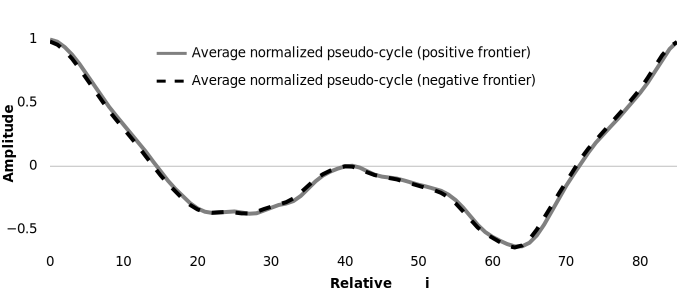
\includegraphics{04averagepc-alto.pdf}
    % \def\svgwidth{\linewidth}
    %\input{01signalenvelope.pdf_tex}
  \caption{Average pseudo-cycles, superimposed, after a change of phase of $-\pi$ on the average pseudo-cycle defined by the negative frontier, for an alto singer digital signal.}
  \label{fig:averagepc-alto}
\end{figure}

Figure \ref{fig:averagepc-alto} makes clear that the average pseudo-cycles for the alto singer signal, as estimated by both frontiers, are in reasonable agreement, despite the evident vertical asymmetries of the underlying wave.

That is not always the case, however, as figure \ref{fig:averagepc-piano33} illustrates. For a discrete signal representing the recording o the key 33 of a grand piano, we can see that the average pseudo-cycle inferred from the positive frontier is substantially different from the one obtained with the negative frontier.

The horizontal lines indicate the maximum of each pseudo cycle, being the point of adjacency between two subsequent pseudo cycles. For the average defined by the negative frontier we see that there is a local maxima near that middle that is almost as high as the global maxima, which is not the case as the average defined by the positive one.

\begin{figure}[ht!]
  \centering
    %  \includegraphics[width=0.9\linewidth]{01signalenvelope}
     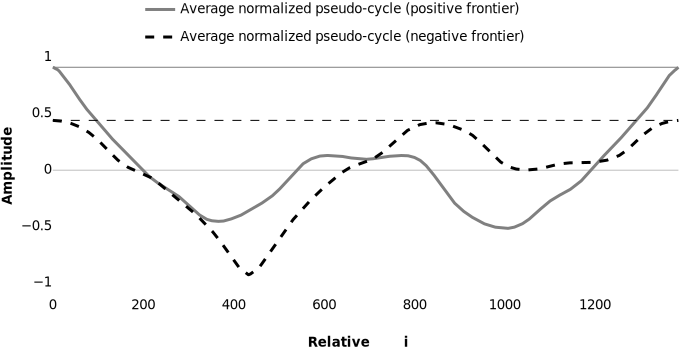
\includegraphics{04averagepc-piano33.pdf}
    % \def\svgwidth{\linewidth}
    %\input{01signalenvelope.pdf_tex}
  \caption{Average pseudo-cycles, superimposed, after a change of phase of $-\pi$ on the average pseudo-cycle defined by the negative frontier, for a grand piano digital signal. The horizontal lines in the figure mark the points of maximum of each of the average pseudo cycles.}
  \label{fig:averagepc-piano33}
\end{figure}

We could take the average of those two representations, but that would dilute the parametric representation of the pseudo-cycle, besides introducing unnecessary complication in the stage of recreating the wave, as we would have to deal with redundant information about the location of each pseudo-cycle.

Instead, a measure of the statistical variance of the lengths of the pseudo cycles will be used in order to select the most appropriate frontier as guide for the construction of the average pseudo cycle waveform.

Figure \ref{fig:std-piano33} shows the distribution of the lengths of the pseudo cycles of the grand piano digital signal. We can use the standard deviation as this measure, and use the pseudo cycles as defined by the frontier with the least standard deviation.

\begin{figure}[ht!]
  \centering
    %  \includegraphics[width=0.9\linewidth]{01signalenvelope}
     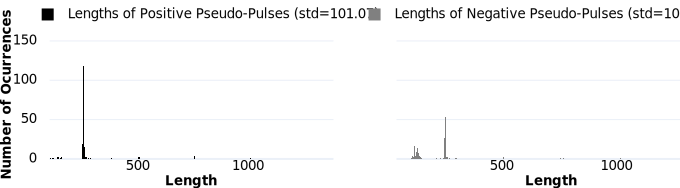
\includegraphics{05std-piano33.pdf}
    % \def\svgwidth{\linewidth}
    %\input{01signalenvelope.pdf_tex}
  \caption{Histogram of the distribution of lengths of the pseudo cycles, as defined by the positive and negative frontiers, and the accompanying standard deviation, for a digital signal of the key 33 of a grand piano.}
  \label{fig:std-piano33}
\end{figure}

Thus, a tillable parametric representation of the average pseudo-cycle can be obtained via the least mean squares method; we are interested in the polynomial that best approximates the average pseudo cycle, respecting the conditions that the beginning and the end of this polynomial must coincide, as must the first derivative of that polynomial in those places, if we are to obtain a smooth transition between pseudo cycles.

From \textcite{2013SelesnickLeast} we know that a constrained least mean squares problem of the form $ \underset{A}{\min} ||Q A - Y||^2_2 \quad \text{subject to} \quad V A = B $ has a closed form approximate solution $ \hat{A} = \left(Q^{T} Q\right)^{-1} \left(Q^{T} Y - V^{T} \left(V \left(Q^{T} Q\right)^{-1} V^{T}\right)^{-1} V \left(Q^{T} Q\right)^{-1} Q^{T} Y - B \right) $, where $ Y $ is the vector we are interested in approximating.

We can proceed to define the real vector $ U = \{ u_0, u_1, \cdots, u_{m-1}\} $ as the average of all normalized pseudo-cycles, with $ m \in \mathbb{N} $ equal to the number of elements and the maximum length of the pseudo-cycles identified by the envelope detection algorithm.

As we are interested in maintaining $ C^0 $ and $ C^1 $ continuity between two adjacent pseudo-pulses, it is convenient to define the vector $ Y $ as two vectors $ E $ stacked, that is $ Y = \{ u_0, u_1, \cdots, u_{m-1}, u_0, u_1, \cdots, u_{m-1}\} $. 

$ A $, the vector of coefficients we are interested in estimating, will thus be composed of $ 2 (k + 1) $ items, where $ k $ is the order of the polynomial to be used in the approximation. Half those values are redundant, however, and $ A $ can thus be defined as $ A = \{ a_0, a_1, \cdots, a_k, a_0, a_1, \cdots, a_k \} $. $ Q $ is formed as usual, with the difference that
it is duplicated horizontally, as seen in equation \ref{eq:matrix}.

Anticipating that we will eventually evaluate this polynomial in various lengths, it is convenient to normalize $ X $ between $ 0 $ and $ 1 $, defining $ X = \left\{ \cancelto{0}{\frac{0}{m-1}}, \frac{1}{m-1}, \frac{2}{m-1}, \cdots, \cancelto{1}{\frac{m-1}{m-1}} \right\} $

\begin{equation} \label{eq:matrix}
\stackrel{Q_{m \times 2 (k + 1)}} {
\begin{bmatrix}
  1      & x_0     & \cdots & x_0^k   & 1      & x_0     & \cdots & x_0^k   \\
  1      & x_1     & \cdots & x_1^k   & 1      & x_1     & \cdots & x_1^k   \\
  \vdots & \vdots  & \ddots & \vdots  & \vdots & \vdots  & \ddots & \vdots  \\
  1      & x_{m-1} & \cdots & x_{m-1} & 1      & x_{m-1} & \cdots & x_{m-1} \\
\end{bmatrix}
}
\stackrel{A_{2 (k + 1) \times 1}}
{
\begin{bmatrix}
a_0    \\
a_1    \\
\vdots \\
a_k    \\
a_0    \\
a_1    \\
\vdots \\
a_k    \\
\end{bmatrix}
}
=
\stackrel{Y_{2 m \times 1}}
{
\begin{bmatrix}
y_0     \\
y_1     \\
\vdots  \\
y_{m-1} \\
y_0     \\
y_1     \\
\vdots  \\
y_{m-1} \\
\end{bmatrix}
}
\end{equation}

To maintain the continuity and smoothness, as well as the identity between the first and second half of the coefficients, $ V $ can be defined as in equation \ref{eq:constraint}.

\begin{equation} \label{eq:constraint}
\stackrel{V_{k + 3 \times 2 (k + 1)}} {
\begin{bmatrix}
  1      & 0       & \cdots & 0           & -1     & 0        & \cdots & 0                \\
  0      & 1       & \cdots & 0           & 0      & -1       & \cdots & 0                \\
  \vdots & \vdots  & \ddots & \vdots      & \vdots & \vdots   & \ddots & \vdots           \\
  0      & 0       & \cdots & 1           & 0      & 0        & \cdots & -1               \\
  1      & x_0     & \cdots & x_0^k       & -1     & -x_{m-1} & \cdots & -x_{m-1}^k       \\
  0      & 1       & \cdots & k x_0^{k-1} & 0      & -1       & \cdots & -k x_{m-1}^{k-1} \\
\end{bmatrix}
}
\stackrel{A_{2 (k + 1) \times 1}}
{
\begin{bmatrix}
a_0    \\
a_1    \\
\vdots \\
a_k    \\
a_0    \\
a_1    \\
\vdots \\
a_k    \\
\end{bmatrix}
}
=
\stackrel{B_{k + 2 \times 1}}
{
\begin{bmatrix}
0      \\
\vdots \\
0      \\
\end{bmatrix}
}
\end{equation}

The initial $k+1$ lines of $V$ assure that the first half of the coefficients of $A$ are equal to the second half, while the penultimate line ensures $C^0$ continuity and the last line ensures $C^1$ continuity, guaranteeing that the derivatives at the beginning and the end of the parametric pseudo cycles are equal.

\begin{figure}[ht!]
  \centering
    %  \includegraphics[width=0.9\linewidth]{01signalenvelope}
     \includegraphics{06approximation-alto}
    % \def\svgwidth{\linewidth}
    %\input{01signalenvelope.pdf_tex}
  \caption{Two adjacent pseudo-cycles. The detail view illustrates that $C^0$ and $C^1$ smoothness are maintained in the parametric representation when two reconstructions are stacked horizontally.}
  \label{fig:05approximation-alto}
\end{figure}



% \begin{table}[ht!]
% \centering
% \begin{tabular}{ l c c }
% \hline
% Method & LMS & time(s) \\
% \hline
% Presented Algorithm & 0.0088 & 4.1507 \\ 
% Smoothing           & 0.0123 & 0.1911 \\ 
% Low pass Filter      & 0.0258 & 0.5601 \\ 
% Hilbert Transform   & 0.0141 & 0.2599 \\ 
% \hline
% \end{tabular}
% \caption{Comparison of the algorithm present in this work with the most common methods of digital envelope identification.}
% \label{table:Comparison}
% \end{table}


\printbibliography

\end{document}
